
В области определения позы животных проделано гораздо меньше работы, чем в этой же области для людей. Причины очевидны:
\begin{itemize}[wide]
    \item Широкий потенциал применения;
    \item Возможность использовать актёров;
    \item Большое количество фотографий.
\end{itemize}
\subsection{На людях} \label{on_people}
Сейчас классификацию позы людей осуществляют с помощью так называемого Pose Estimation Tree. Целью зрения становится по изображению будто восстановить человеческий скелет. Для этого определяются важные подвижные узлы - joints, см рисунок \ref{img:poseest}  . Обычно ими являются локти, колени и другие суставы. У человека всего порядка 200 таких узлов. При этом при решении большинства задач компьютерного зрения используется около 20.
\begin{figure}[ht] 
  \center
  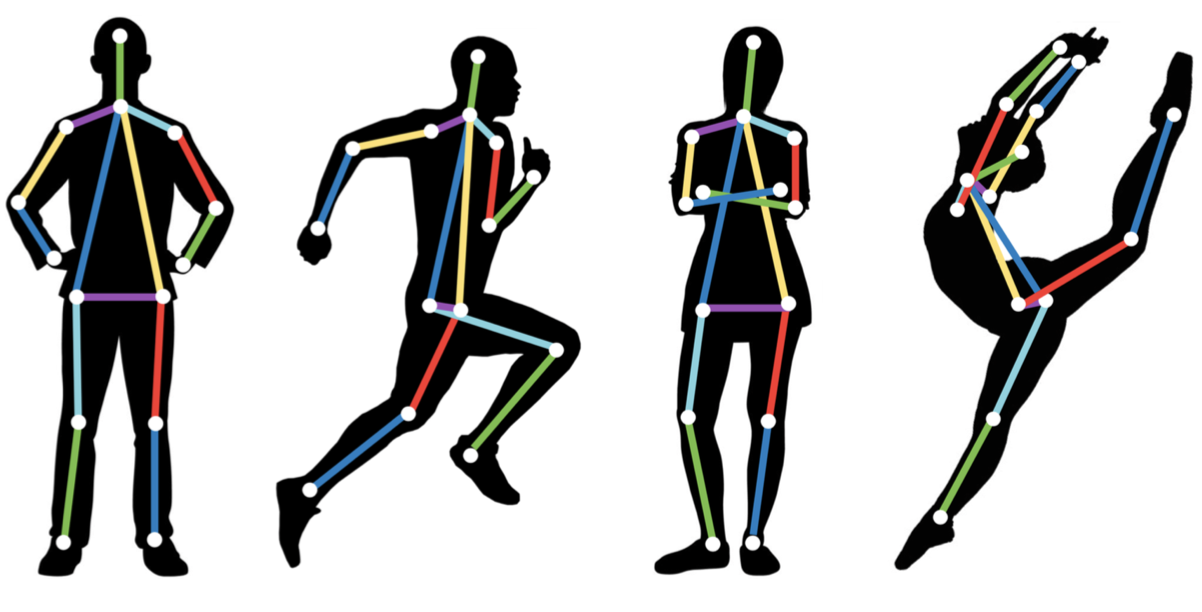
\includegraphics [width=\textwidth/2] {pose}
  \caption{Pose Estimation Tree} 
  \label{img:poseest}  
\end{figure}

Классические пакетные решения для такой задачи - Tensorflow Pose Kit и OpenPose\cite{openpose}. Всё, что требуется для этих пакетов - набор размеченных данных для обучения. 

OpenPose может работать с множественными объектами и окклюзиями, но относительно медленный. Tensorflow Pose Kit создан с уклоном в перенос модели на портативные устройства.

Согласно статье Эми Берман\cite{Bearman2015HumanPE}, даётся совет использовать классификацию деятельности строго отдельно от задачи получения дерева конечностей человека, а не одно на результатах другого. Основная причина в том, что дерево конечностей крайне нестабильно, его точность далека от идеальной и от окклюзий конечностей самим человеком практически нельзя избавиться. В подтверждение этому, на 20 классах активности они добились точности в 80\% без использования pose estimation, что считается хорошо для такого большого количества классов.

\subsection{На животных} \label{on_animals}
В 2018 году вышла публикация \cite{deeplabcut}, в которой авторы предложили новаторский способ автоматически следить за указанными частями тела у животных. Алгоритму не требуется больших датасетов с данными, нужно всего около 200 кадров (от 8 секунд видео) чтобы предсказать остальной видеопоток. Пример работы DeepLabCut виден на рисунке \ref{img:deeplabcut}.
\begin{figure}[ht] 
  \center
  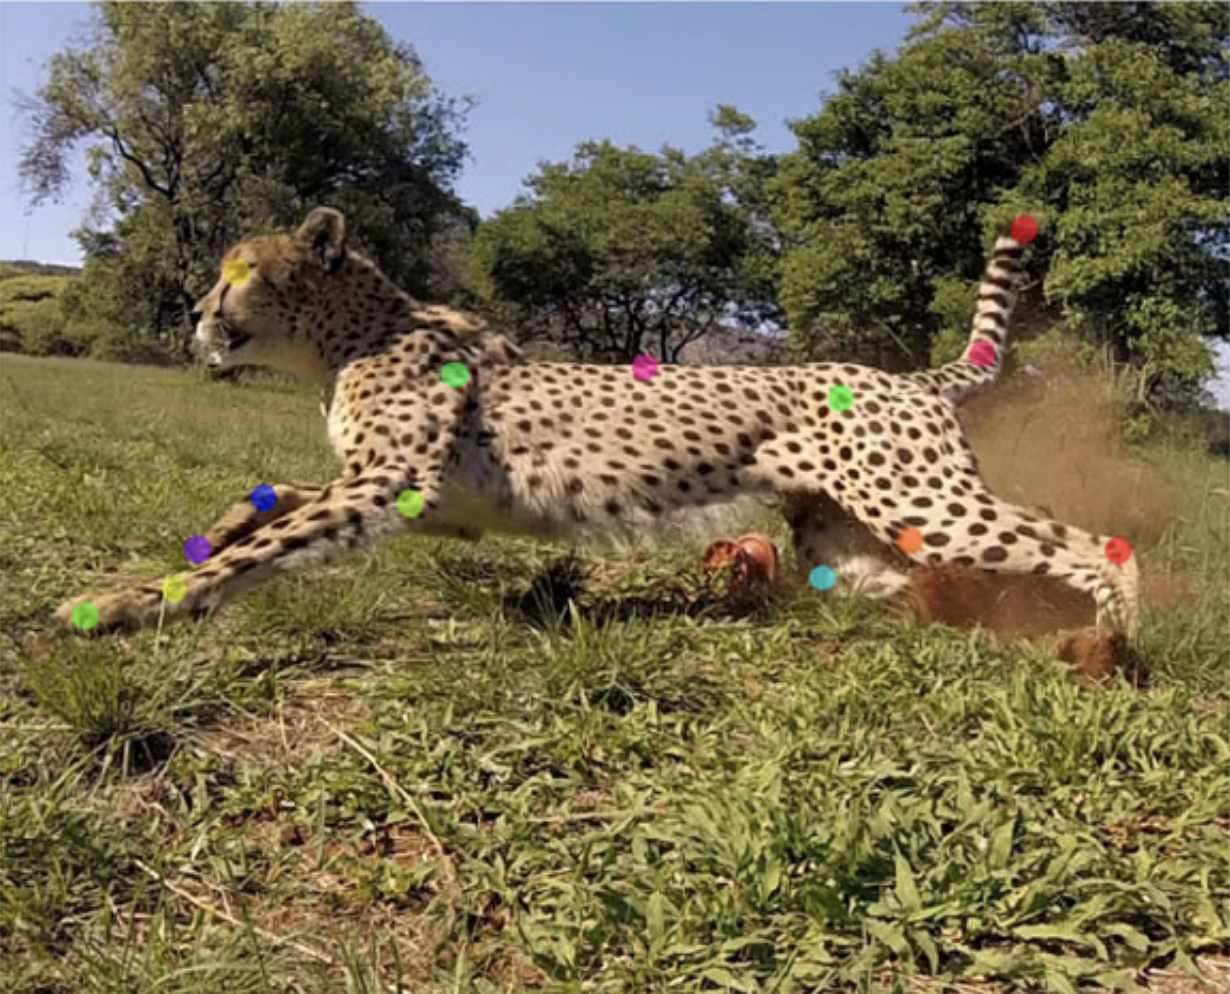
\includegraphics [width=\textwidth/2] {deeplabcut}
  \caption{Предсказанный кадр DeepLabCut} 
  \label{img:deeplabcut}  
\end{figure}

Ограничениями данного метода являются два момента. И первый из них - необходимость в разметке этих первых 200 кадров, на это уходит обычно около 20 минут. Второй - принципиальная возможность работать только с видеопотоком.

В итоге это достаточно хороший метод для того, чтобы разметить большие видеопотоки. Алгоритм обеспечивает достаточную точность и на длинных видеозаписях позволяет сильно сократить время на разметку данных для Pose Tree Estimation. 

Применение данного способа не ограничивается только на животных: любой видеопоток, на котором можно отслеживать объекты, будет работать.

\subsection{Скелетонизация} \label{skeletonization}
Если контуры объектов отчётливо видны, часто можно вместо решения тяжёлой задачи Pose Estimation решить проблему локализации конечностей более простыми алгоритмами. Одним из таких является скелетонизация\cite{skeletonization}. Наглядно принцип работы алгоритма представлен на рисунке \ref{img:skeleton}.

\begin{figure}[ht] 
  \center
  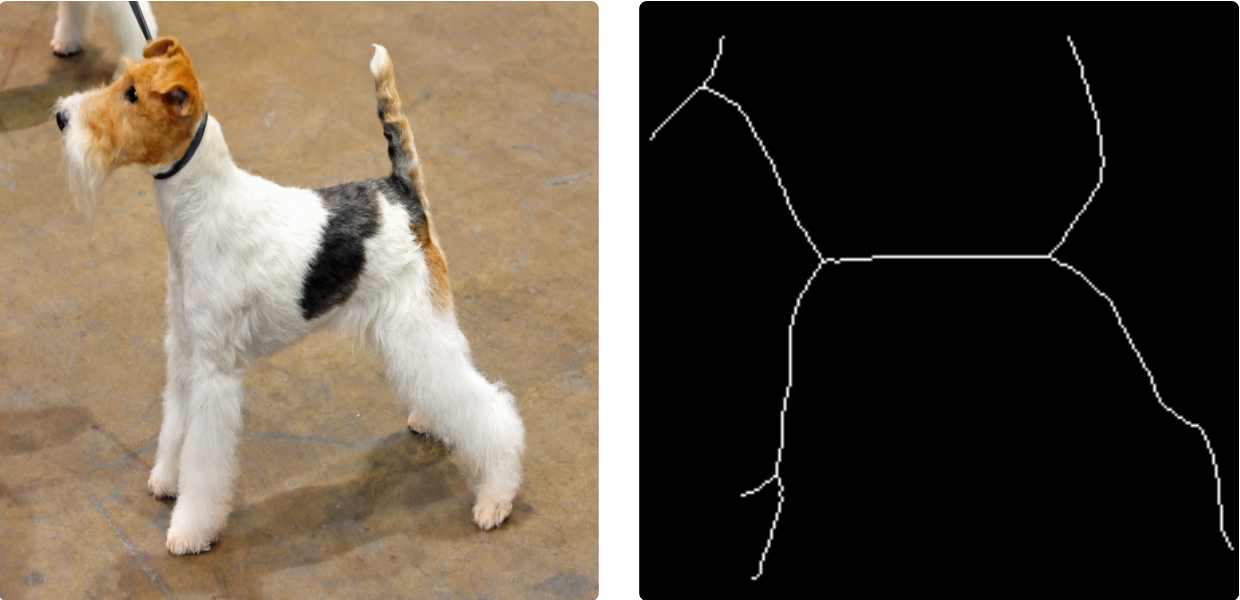
\includegraphics [width=\textwidth/2] {skeletonization}
  \caption{Скелетонизация} 
  \label{img:skeleton}  
\end{figure}

Этот алгоритм не требует данных для обучения, всё что ему требуется - это маска объекта. То есть бинарное изображение контура собаки. Алгоритм уменьшит толщину этого контура до одного пикселя.

Недостатки этого метода видны на изображении. Если несколько конечностей не разделены пустым пространством, этот метод распознает их за одну.